\section{Angular}


\subsection{Elements}

\begin{itemize}
    \item \emph{Element}: Wrapper around \inlinecode{nativeElement}. Wrapped so as to abstract away differences between native elements in browser and on mobile.
    \item \emph{View}: Smallest group of elements that are created and destroyed together.
        \begin{itemize}
            \item HostView: A view created by a component
            \item EmbeddedView: A view created by a template
        \end{itemize}
    \item \emph{Component}
    \item \emph{Directive}: An attribute that may be appended to a component. Like a component, but without an html-file.
    \item \emph{Template}: Angular-html-files are usually static. The only dynamics that are allowed are via subcomponents or templates \inlinecode{<ng-template>}. Templates are really like simple, inline html-only subcomponents. They are even more like inline-functions in that they have access to their parent-component's template-variables.
    \item \emph{ViewContainer}: removing html-elements from the DOM is dangerous, because angular will not be aware of that removal - it will keep the node in memory and continue running change detection. So how do you remove elements? That's what ViewContainers are for: wrapping a node in a ViewContainer provides us with an API to add or remove components or templates.
\end{itemize}

\subsection{Life cycle}

\subsection{Change detection}
Change detection goes top down: if a user-interaction happened on component X, then the whole tree starting at app-root is updated.
If component X has \inlinecode{changeDetectionStrategy: OnPush}, then X and its children are shielded from updates from outside of X's subtree. But events originating from X or its children still traverse the \emph{whole} tree from app-root down.

\subsection{Service availability}
Services are by default provided by app-root. The instance is used by every child component - except if that child, lets call it X, has its own provided instance of the service. Then all children of X use X's instance of the service.


\subsection{Building blocks}

\begin{itemize}
    \item The \emph{compiler} 
        \begin{itemize}
            \item Runs offline and is not included in the bundled application (except when in development mode).
            \item Takes \inlinecode{*.component.ts} and \inlinecode{*.component.html} files and turns them into a \inlinecode{*.ngfactory.ts} file.
            \item The \inlinecode{*.ngfactory.ts} file contains a \inlinecode{ComponentDef} class with a \inlinecode{factory} method and a \inlinecode{template} method.
        \end{itemize} 
    \item The \emph{runtime}: \inlinecode{core.js/tick()} 
        \begin{itemize}
            \item Module bootstrap
            \item View creation
                \begin{itemize}
                    \item Instantiates a view by calling \inlinecode{const viewDef = compDef.factory(depInjector)} 
                        \begin{itemize}
                            \item A ViewDef has a list of nodes \inlinecode{viewDef.nodes[]}
                            \item Nodes can be accessed as \inlinecode{ElementRef}, \inlinecode{TemplateRef} or \inlinecode{ViewContainerRef}
                            \item A ViewDef has a \inlinecode{template()} method that calls render-functions like \inlinecode{text()}, \inlinecode{heading()}, \inlinecode{div}, ...
                        \end{itemize}
                    \item Calls the ViewDef's template-function \inlinecode{viewDef.template()}
                \end{itemize}
            \item Change detection 
                \begin{itemize}
                    \item 
                \end{itemize}
        \end{itemize}
\end{itemize}


The different parts of an angular application are namespaced in an interesting way.
\begin{itemize}
    \item The \emph{compiler} inspects html-files and writes components, directives and pipes into them
    \begin{itemize}
        \item Components, directives and pipes are namespaced in \emph{modules}
    \end{itemize}
    \item The \emph{injector} injects services and guards into components
    \begin{itemize}
        \item Services and guards are not namespaced - they are always provided in one big pool in app-root.
        \item If you really need to namespace services, there is the \inlinecode{forRoot()} hack.
    \end{itemize}
\end{itemize}


\begin{figure}
    \caption{Angular modules}
    \centering
    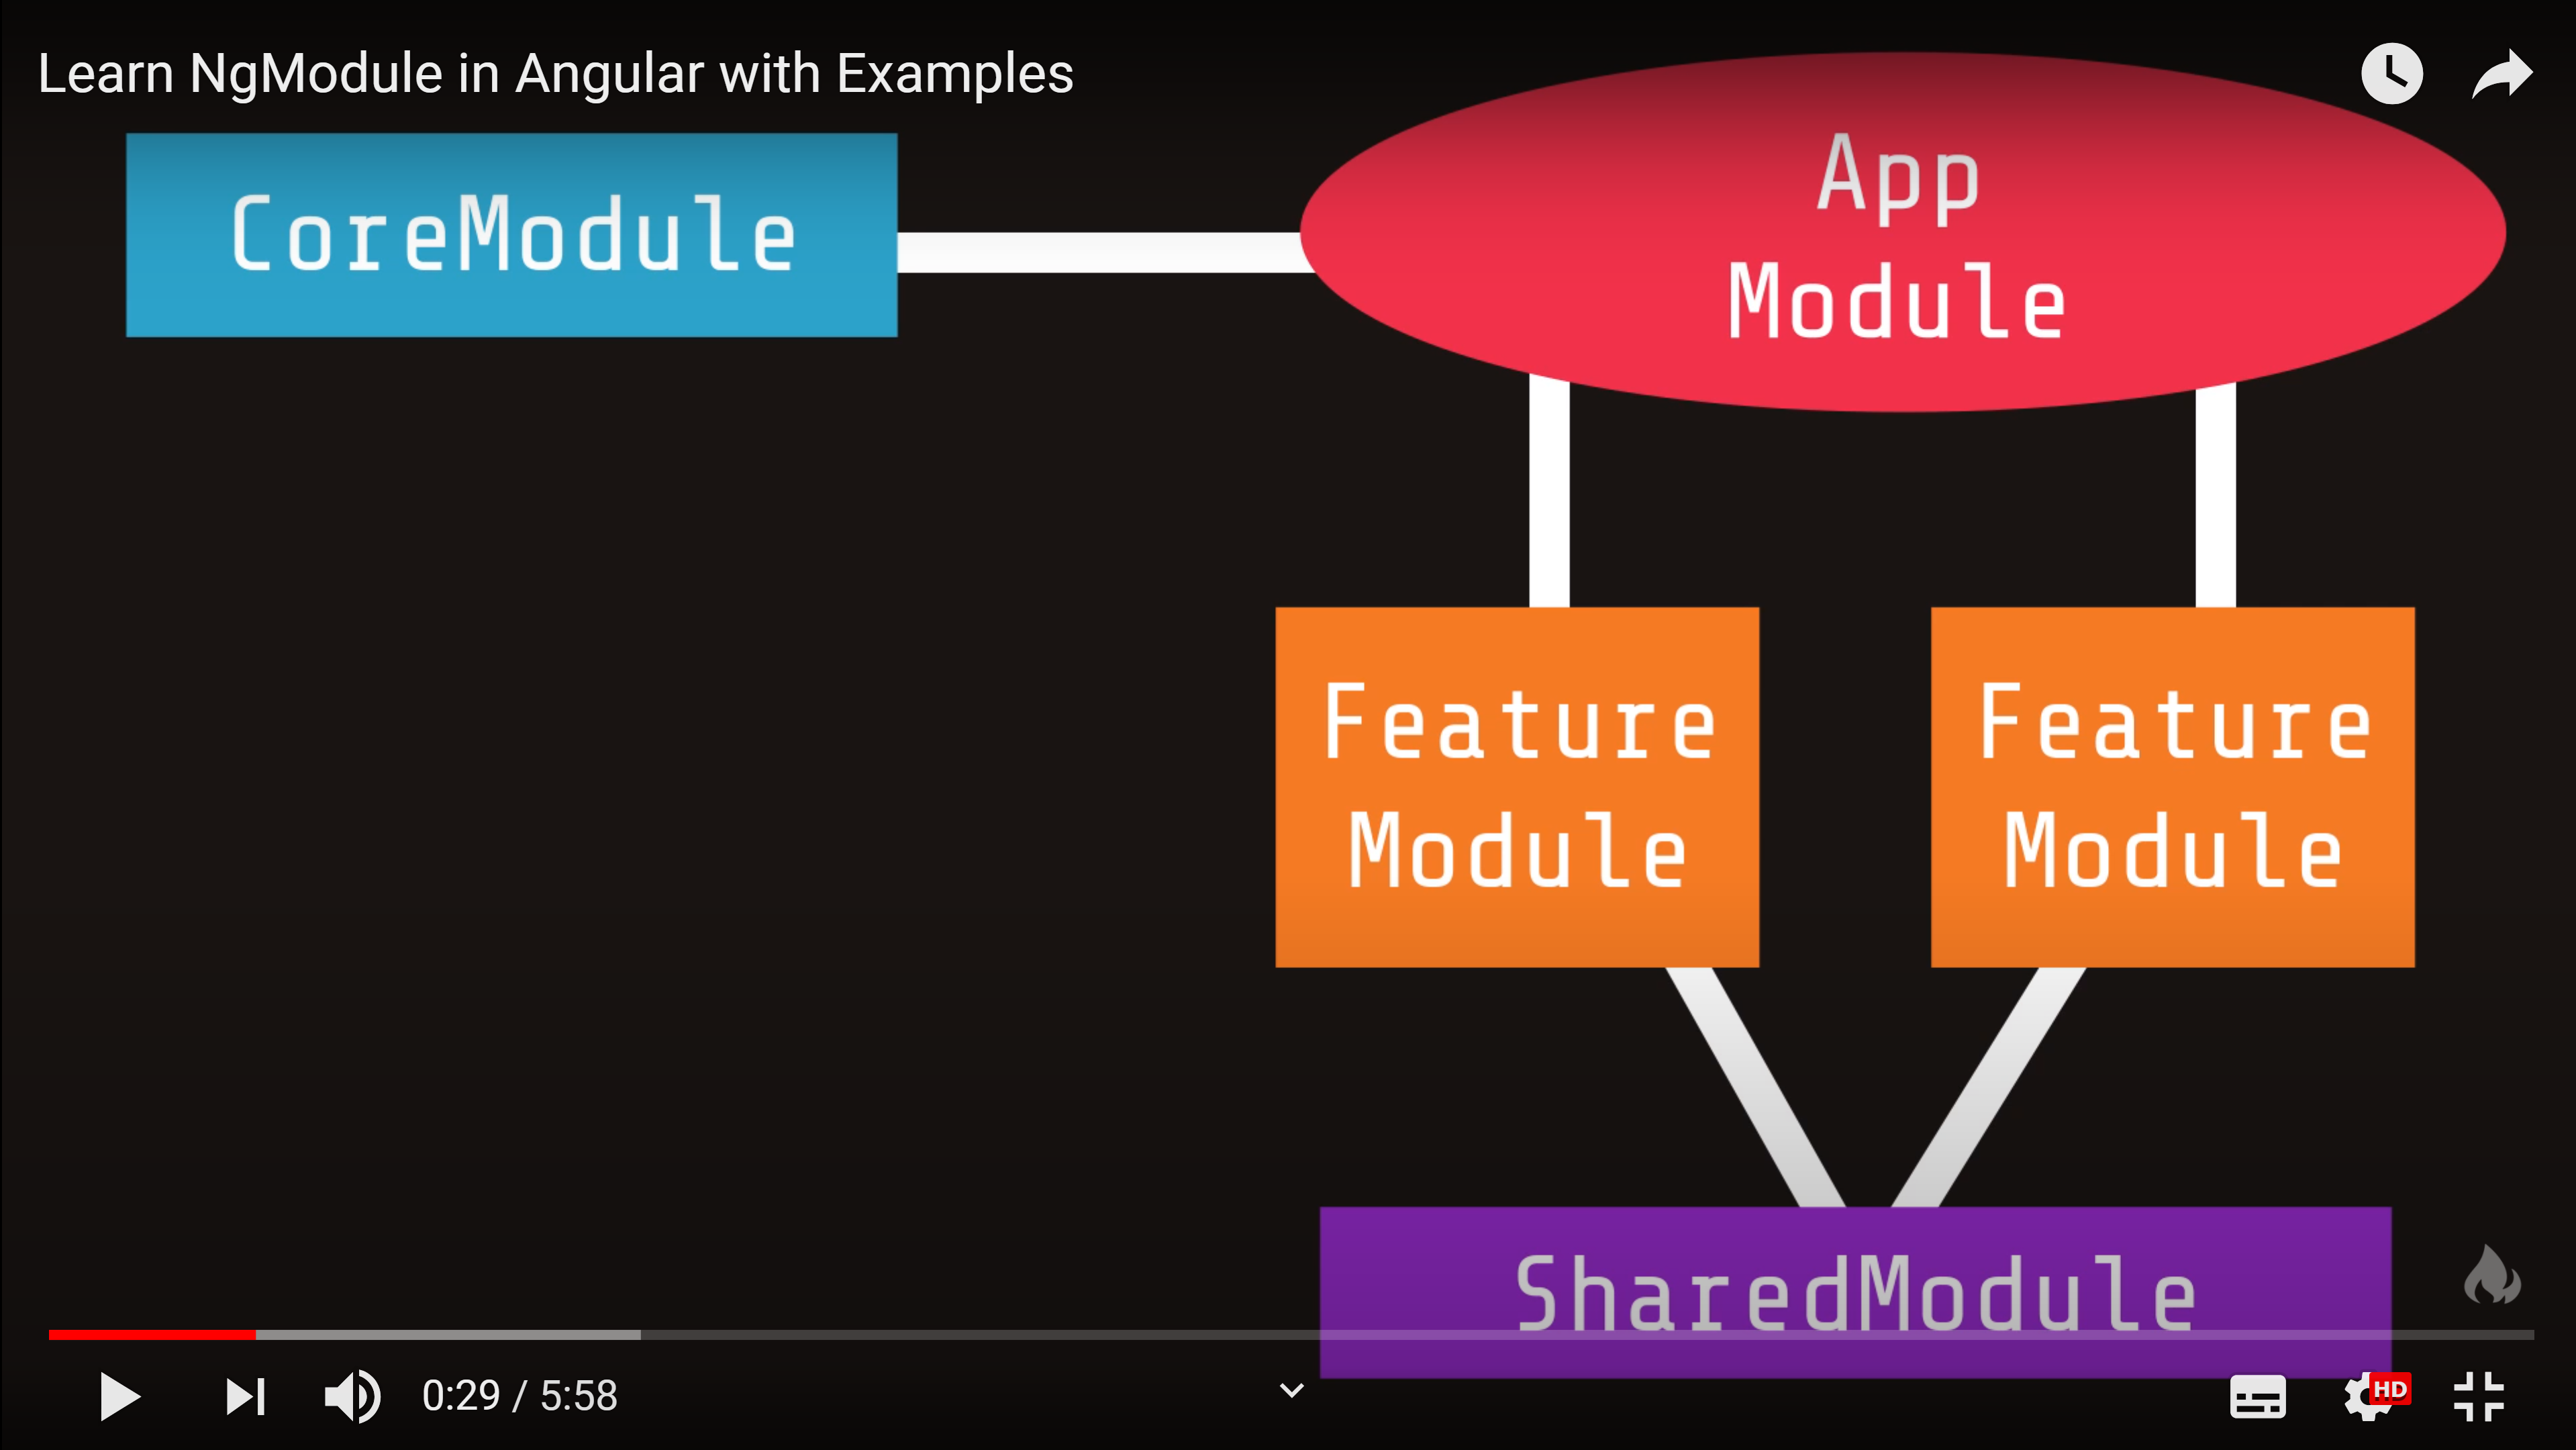
\includegraphics[width=0.5\textwidth]{images/angular_modules.png}
\end{figure}

\begin{itemize}
    \item app module: root. \inlinecode{imports} other modules and \inlinecode{bootstrap}'s the root-component.
    \item core module: exports shared singleton services and guards in its \inlinecode{providers}. Should be imported only in app-module.
    \item feature module: exports thematic components, directives and pipes in its \inlinecode{declarations} and \inlinecode{exports}. Should be imported only in app-module.
                If necessary, feature modules may provide services, but then you need to make sure that the module is only imported in one single place (usually the app-module).
    \item shared module: exports globally used components, directives and pipes in its \inlinecode{declarations} and \inlinecode{exports}. Should be imported into any module that requires it.
                Shared modules \emph{must not} export services, because they are imported in several other modules. The presence of the same service in multiple modules will have the injector commit harakiri.
    \item router module: imported into app module. Side-effect-configures the angular-core-router using \inlinecode{forRoot}.
\end{itemize}